\chapter{Large-eddy simulation of wind farms: methodology}\label{ch:methodology}


This chapter discusses the large-eddy simulation methodology for the numerical simulation of the atmospheric boundary layer, and the evaluation of wind-farm power extraction. The in-house SP--Wind framework is used, developed over the years at KU Leuven (see, e.g., \citealp{meyers2007evaluation, delport2009constrained, calaf2010large, goit2015optimal, allaerts2017boundary}). Firstly, Section~\ref{sec:meth_governing} introduces the equations governing the boundary-layer flow. Thereafter, Section~\ref{sec:meth_adm} details the actuator disk wind turbine model used throughout this thesis. Subsequently, Section~\ref{sec:meth_discr} elaborates on the numerical discretization schemes applied to the continuous governing equations. Section~\ref{sec:meth_fringe} introduces the fringe region technique used to impose non-cyclic inlet boundary conditions. Finally, Section~\ref{sec:meth_par} illustrates the novel parallelization strategy implemented in the flow solver in order to reduce simulation wall times, and highlights computational performance aspects. 

\section{Governing equations}\label{sec:meth_governing}
The wind-farm boundary layer flows considered in this thesis are modeled through the unsteady incompressible Navier-Stokes equations, solved by means of an LES strategy. This strategy entails that the large energy-containing motions in the turbulent boundary layer flow, which are most important for energy extraction, are resolved with adequate spatio-temporal resolution, whereas the small-scale dissipative fluctuations in the flow are represented by a subgrid-scale model. The resulting governing equations are the filtered incompressible Navier-Stokes momentum and continuity equations: 
\begin{align}
	\frac{\partial \ufilt}{\partial t} + (\ufilt \cdot \nabla) \ufilt &= -\nabla (p_\infty + \tilde{p}^\star) - \nabla \cdot \blds{\tau}_{\text{sgs}} + \sum_{i=1}^{N_t} \blds{f}_i, \label{eq:NSmomentum}\\ 
 	\nabla \cdot \ufilt &= 0. \label{eq:NScontinuity}
\end{align}

In these equations, $\ufilt = [\tilde{u}_x, \tilde{u}_y, \tilde{u}_z]$ is the three-dimensional velocity field filtered at the grid scale, with $x$, $y$, and $z$ indicating the streamwise, spanwise, and vertical direction respectively. The force $\bs{f}_i$ enacted by turbine $i$ (out of $N_t$ turbines) on the boundary layer flow is parametrized using an actuator disk approach, detailed in Section~\ref{sec:meth_adm}. The flow is forced through the domain with a constant imposed background pressure gradient $\nabla p_\infty = [\partial_x p_\infty/\rho, 0, 0]$, defining a friction velocity $u_* = - \sqrt{H \partial_x p_\infty/\rho}$ as a velocity scale representative for the shear stress enacted by the ground surface on the flow, and a reference time scale $t_* = H/u_*$, with $H$ the height of the simulation domain, and $\rho$ the density of air. 

The subgrid-scale (SGS) stress tensor $\blds{\tau}_{\text{sgs}} = \widetilde{\blds{u} \blds{u}} - \ufilt \ufilt$ represents the effect of momentum transport caused by unresolved turbulent motions on the resolved scales. As is standard practice in incompressible LES, the trace of this tensor is absorbed into the modified filtered pressure $\tilde{p}^\star = \tilde{p}/\rho - p_\infty / \rho + \text{tr}(\bs{\tau}_\text{sgs})$. In the remainder of this text, the $^\star$ notation is omitted, and $\ptilde$ denotes the modified filtered pressure. Its deviatoric part is modeled using a standard constant-coefficient eddy-viscosity Smagorinsky model as 
\begin{equation}
	\blds{\tau}_{\text{sgs}} = - 2 \lambda^2 (2 \blds{\mathcal{S}} : \blds{\mathcal{S}})^{1/2} \blds{\mathcal{S}},
\end{equation}
where $\blds{\mathcal{S}} = \big(\nabla \ufilt + (\nabla \ufilt)^T \big)/2$ is the rate-of-strain tensor \citep{smagorinsky1963general}. Furthermore, the Smagorinsky length scale is parametrized as $\lambda = C_s \Delta$ away from the wall, with a constant Smagorinsky coefficient $C_s$, and the local grid scale $\Delta = (\Delta_x \Delta_y \Delta_z)^{1/3}$. The Smagorinsky length scale $\lambda$ is damped near the bottom ground wall to avoid excessive dissipation of kinetic energy using the damping function introduced by \cite{mason1992stochastic}, i.e. $\lambda(z)^{-n} = [C_s \Delta]^{-n} + [\kappa (z + z_0)]^{-n}$, with $\kappa = 0.4$ the Von Karman constant, $z_0$ the assumed roughness length at the wall. Throughout the current work, we use $C_s = 0.14$ and $n = 1$, as this leads to suitable dissipation characteristics for the high Reynolds number boundary-layer simulations in this thesis \citep{meyers2011error}.

The large Reynolds numbers associated with atmospheric flows at the wind-farm scale justify the omission of resolved effects of viscosity. Furthermore, Coriolis and thermal stratification effects are also omitted. This entails that, throughout this thesis, an infinite-Reynolds-number rough-wall half-channel flow is used as a surrogate for the ABL. Although Coriolis and stratification effects can be important for overall wind-farm behavior (see, e.g. \citealp{allaerts2015large, allaerts2017boundary}), the extent to which these effects can be exploited in optimal control of wind-farm boundary layers remains an open question which is outside the scope of the current work. 

Figure~\ref{fig:les_field} illustrates a snapshot of a wind-farm LES using typical setup parameters for this thesis. It can be seen from the figure that the LES resolves the large-scale energetic flow structures, and is able to capture the complex three-dimensional wake behavior including meandering, turbulent mixing, and interactions with downstream turbines.

\begin{figure}
	\centering
	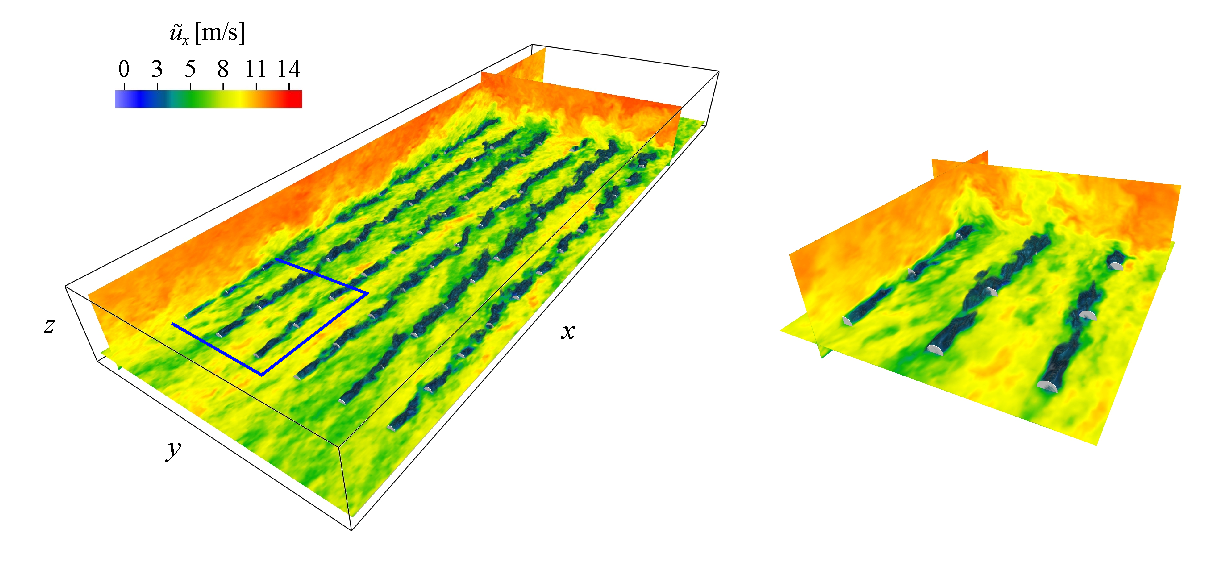
\includegraphics[width=\linewidth]{chapters/methodology/les_field.eps}
	\caption[Snapshot of streamwise velocity of a typical wind-farm LES used in this thesis.]{Snapshot of streamwise velocity of a typical wind-farm LES used in this thesis. Turbines are shown as gray actuator disks. Wakes are rendered as 3D volumetric structures. \emph{Left: } Full wind-farm flow field. \emph{Right: } close-up of flow field indicated in by blue lines on left. Details of simulation setup correspond to Table~\ref{tab:setup_params_ind}. \label{fig:les_field}}
\end{figure}

\section{Actuator disk wind turbine model}\label{sec:meth_adm}
The wind turbines are represented in the simulation domain using a non-rotating actuator disk model (ADM). This approach is chosen as the ADM accurately represents wake behavior except for the very near wake ($x/D < 3$), and as it involves only minor additional requirements on spatiotemporal resolution compared to an ABL without turbines \citep{mikkelsen2003actuator, wu2015modeling}. The non-rotating ADM exerts an exclusively axial thrust force on the flow field. Firstly, the parametrization of this force using a disk-based thrust coefficient will be discussed. Thereafter the calculation of extracted power is elaborated. The section is concluded with a discussion on the control parameters of the actuator disk turbines.

\subsection{Wind turbine thrust force}
Following the approach of \cite{meyers2010large} and \cite{calaf2010large}, the magnitude of the axial thrust force enacted on the flow field by a turbine $i$ is parametrized as 
\begin{equation}
f_i(t) = - \frac{1}{2}~\ctihat(t)~V_{i}^2(t)~A_i,
\end{equation}
where $\ctihat$ is the disk-based thrust coefficient (see discussion on wind turbine controls below). Further, $A_i$ is the rotor area, and $V_i$ is the disk-averaged velocity. As indicated, this force is aligned with the rotor-perpendicular direction, defined as $\eperpi =  \cos \theta_i \bs{e}_x + \sin \theta_i \bs{e}_y $, with $\theta_i$ the yaw angle of the rotor. The force is distributed to the LES grid as 
\begin{equation}
\blds{f}_i(\blds{x},t) = - \frac{1}{2}~\ctihat(t)~V_{i}^2(t)~\mathscr{R}_i(\blds{x})~\eperpi,\label{eq:define_force}, 
\end{equation}
using the spatial kernel $\mathscr{R}_i (\blds{x})$ first introduced by \cite{meyers2010large}, representative of the geometric footprint of turbine $i$ on the LES grid, defined as 
\begin{equation}
\R_i(\bs{x}) = \sint G(\bs{s}-\bs{x}) ~ \diracdelta [(\bs{s}-\bs{t}_i)\cdot\eperpi] ~ H(D/2-\vert\vert \bs{s}-\bs{t}_i\vert\vert_2) \ds \label{eq:R}.
\end{equation} 
In this definition, $G(\bs{y}) = [6/(\pi \Delta_f)]^{3/2} \exp(-6\vert\vert \bs{y}\vert\vert_2^2/\Delta_f^2)$ is a three-dimensional Gaussian filter with a filter width $\Delta_f = 3/2\Delta$, $H$ is the Heaviside function and $\diracdelta$ the Dirac delta function. Further, $\bs{t}_i$ represents the hub coordinates of turbine~$i$ and $D$ is its rotor diameter. As shown in Figure~\ref{fig:Rkernel}, this definition leads to a diffuse and smooth representation on the simulation grid, which is amenable to the spectral discretization methods discussed further below. Note that, by definition, $\sint \R_i \dx = A_i$.

The disk-averaged velocity $V_i$ is calculated using the same geometric footprint $\R_i$ as 
\begin{equation}
V_{i} = (1/A_i) \int_\Omega \mathscr{R}_i(\blds{x})\ \ufilt \cdot \eperpi \ \dx.
\end{equation} 
A slight difference of the current ADM with the aforementioned studies of \cite{meyers2010large} and \cite{calaf2010large} is the omission of a time-filtering operation on the disk velocity $V_i$ here. 

\begin{figure}
	\centering
	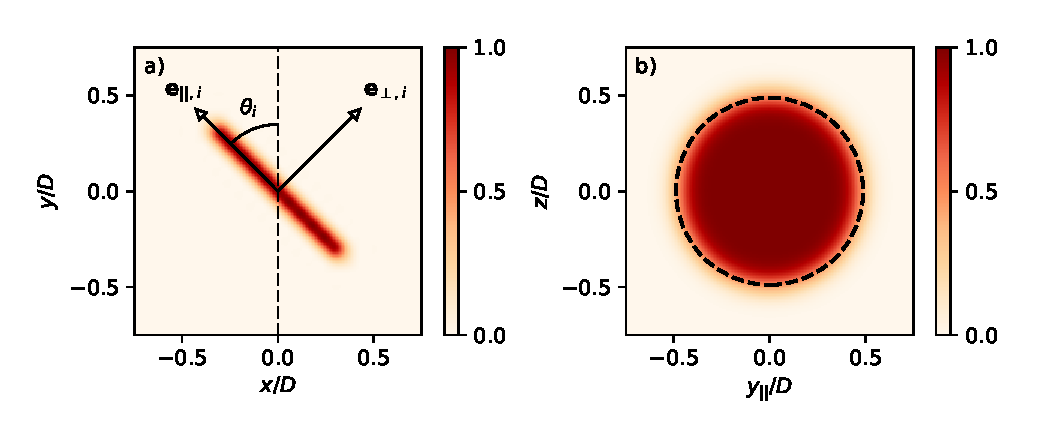
\includegraphics[width=\textwidth]{chapters/methodology/visualize_R.eps}
	\caption[Visualization of geometric footprint $\R$ of actuator disk turbine with yaw angle $\theta_i = 45^\circ$ on LES grid.]{Visualization of geometric footprint $\R$ of actuator disk turbine with yaw angle $\theta_i = 45^\circ$ on LES grid. \emph{a)} Topview. \emph{b)} Cross-section through rotor plane. Coloring normalized by maximum value of $\R$. \label{fig:Rkernel}}
\end{figure}

\subsection{Wind turbine power extraction}
The mechanical power captured by the wind turbine is calculated as 
\begin{align}
P_i(t) &= \frac{1}{2} C_{P,i}'(t)~V_{i}^3(t)~A_i = \frac{1}{2}~a\ctihat(t)~V_{i}^3(t)~A_i.\label{eq:define_power}
\end{align}
In contrast to earlier work applying ADM turbines in wind-farm LES \citep{meyers2010large, calaf2010large, goit2015optimal}, where $C_P' = \widehat{C}_T'$, here the disk-based power coefficient $C_{P,i}' = a\widehat{C}_{T,i}'$, with $a = 0.9$ the result of fitting LES results to one-dimensional momentum theory as described in Appendix~\ref{ch:app_adm}. This is done in order to eliminate overpredictions in power extraction observed using turbine parametrizations on typical wind-farm grid resolutions (see, e.g. \citealp{martinez2016wind, martinez2015large}), which are caused by an overestimation of $V_i$ due to a spill-over effect of the footprint $\R_i$ over the rotor perimeter (see Figure~\ref{fig:Rkernel}b). Remark that, due to the linear nature of this fit, it does not influence results on power extraction discussed throughout this work, as they are always normalized by a reference power. 

\subsection{Wind turbine controls}
Wind turbines are controlled dynamically in such a way as to actively influence the turbulent ABL flow and yield favorable conditions for farm-aggregated power extraction. This influence originates from the thrust force enacted by the turbine upon the flow, characterized by its magnitude and orientation. 
As discussed in Chapter~\ref{ch:introduction}, the main features to be controlled in modern horizontal-axis wind turbines are the blade pitch angle $\beta$ using pitch actuators, the tip speed ratio $\lambda$ by varying resisting generator torque, and the yaw angle $\theta$ using the active yaw system. Blade pitch and tip speed ratio influence axial induction behavior, and thus the magnitude of the thrust force, whereas yaw governs the orientation of the thrust force. 

\subsubsection{Axial induction control}
In the context of the ADM used throughout this thesis, the effects of blade pitch $\beta$ and tip speed ratio $\lambda$ on the axial induction are represented through the modified thrust coefficient $\widehat{C}_T'$ (as used in Equation~\ref{eq:define_force}). Following \cite{goit2015optimal}, in the current approach we provide a thrust coefficient setpoint $C_T'$ and make abstraction of how such a setpoint should be attained through variations in $\beta$ or $\lambda$.\footnote{Note that virtually every feasible thrust setpoint can be achieved by multiple ($\beta$,$\lambda$) combinations (see Figure \ref{fig:WT_drawing}c), and that unsteady variations can hence also be achieved in multiple ways.} We do not directly impose the thrust setpoint on the turbine, but instead apply a first-order exponential time filter:
\begin{equation}
	\tau \ddt{\ctihat} = \cti - \ctihat \label{eq:timefilter_def}.
\end{equation}
In this equation, the time constant $\tau$ characterizes the turbine response time to variations in thrust setpoints. This would, for example, fit in a hierarchical approach to wind-farm control, in which wind-farm control signals are passed on to individual turbine controllers that themselves may not react instantaneously to the control signals. Moreover, increasing $\tau$ allows to assess the effect on power gains of limiting dynamics in turbine operation, which could be beneficial for turbine lifetime. 



%\begin{figure}
%	\centering
%	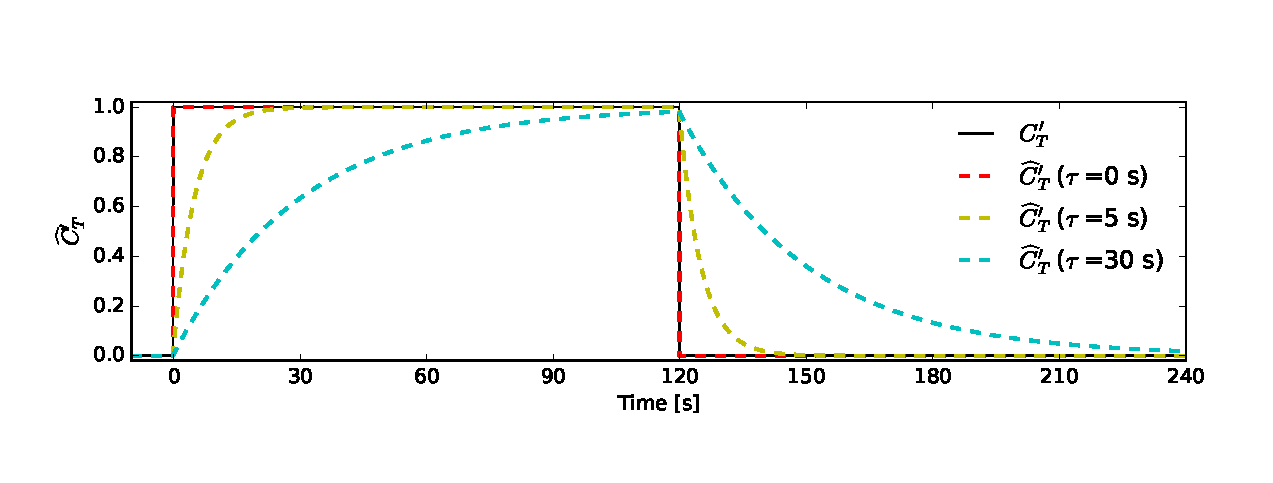
\includegraphics[width=\textwidth]{chapters/optimal_control_problem/figure3.eps}    
%	\caption{Illustration of the response of the thrust coefficient $\widehat{C}_T'$ to a square wave variation in the control signal $C_T'$ for varying wind turbine response times $\tau$. \label{fig:cthat}}
%\end{figure}

In the remainder of this section, we discuss steady-state turbine operation, hence $C_T'$ and $\widehat{C}_T'$ can be used interchangeably. Using relations from 1D momentum theory for an ideal turbine \citep{burton2001wind}, straightforward algebraic manipulation relates the disk-based thrust coefficient $C_T'$ with the conventional power coefficient $C_P$ and thrust coefficient $C_T$ based on undisturbed velocity $V_\infty$ as
\begin{equation}
C_P = 64\frac{C_T'}{(C_T' + 4)^3} \qquad \text{and} \qquad C_T = 16\frac{C_T'}{(C_T' + 4)^2}.
\end{equation}
As shown in Figure~\ref{fig:ct_cpct}, $C_P$ achieves a maximum at the well-known Betz limit of $16/27 \approx 0.593$, for which $C_T' = 2$. This optimal setting, which maximizes individual turbine power, is refered to as \emph{greedy} control, and is used as a reference case throughout this work. In order to obtain any lower $C_P$ value, two possible $C_T'$ setpoints can be chosen: an underinductive ($C_T' < 2$) and an overinductive ($C_T' > 2$) coefficient. Furthermore, it is worth noting that $C_P$ is quite insensitive to $C_T'$ in the range 1.5 to 2.5 indicating that, in this zone, turbine thrust forces can be varied significantly without sacrificing a lot of power. 

\begin{figure}
	\centering
	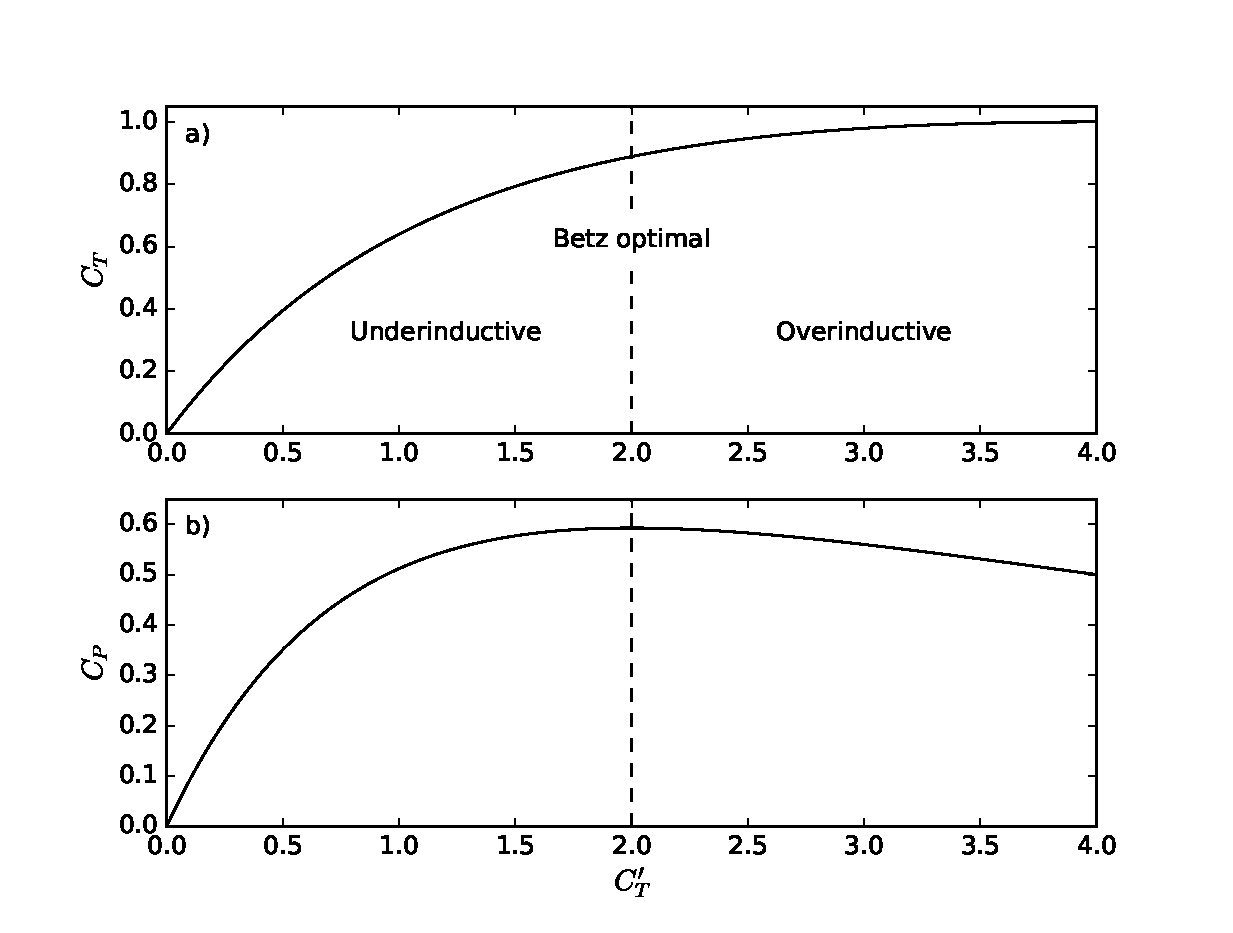
\includegraphics[width=\linewidth]{figures/meth_ct_ctprime_cp.eps}
	\caption[Thrust coefficient $C_T$ and power coefficient $C_P$ as a function of modified thrust coefficient $C_T'$ for a steady turbine based on 1D momentum theory.]{Thrust coefficient $C_T$ (\emph{a}) and power coefficient $C_P$ (\emph{b}) as a function of modified thrust coefficient $C_T'$ for a steady turbine based on 1D momentum theory.}
	\label{fig:ct_cpct}
\end{figure}

For reasons of technical feasibility, we limit \emph{a priori} the thrust coefficient setpoint $C_T'$ by box constraints. On one hand, a lower bound of $C_T' = 0$ prevents the turbine from operating as a fan. On the other hand, we estimate the maximum attainable $C_T'$ based on Figure~\ref{fig:Ct_Uinfty}. This figure contains results of blade element momentum theory calculations for the maximum attainable $C_T'$ for region II operation through increase of the tip speed ratio $\lambda$, using the NREL 5-MW turbine specifications \citep{jonkman2009definition}. The calculations are performed in region II operation at below-rated wind speeds, in which $\lambda$ is conventionally controlled through regulation of the turbine generator torque. It can be seen that in this way, for typical wind conditions of $V_\infty \approx 8$ m s$^{-1}$, a $C_T'$ of approximately 2.5 is feasible. This value could still be increased, e.g. through a minor increase in blade chord length in the design phase of the turbine. Therefore, we consider an ultimately achievable upper bound of $C_T' = 3$ throughout this work.\footnote{Note that, in Chapters~\ref{ch:opt_induction} and~\ref{ch:opt_yaw}, we will also consider underinductive cases, for which we impose an upper limit of  $C_T' = 2$.} Note that this is slightly lower than the maximum value of $C_T' = 4$ applied in \cite{goit2015optimal}.

\begin{figure}
	\centering
	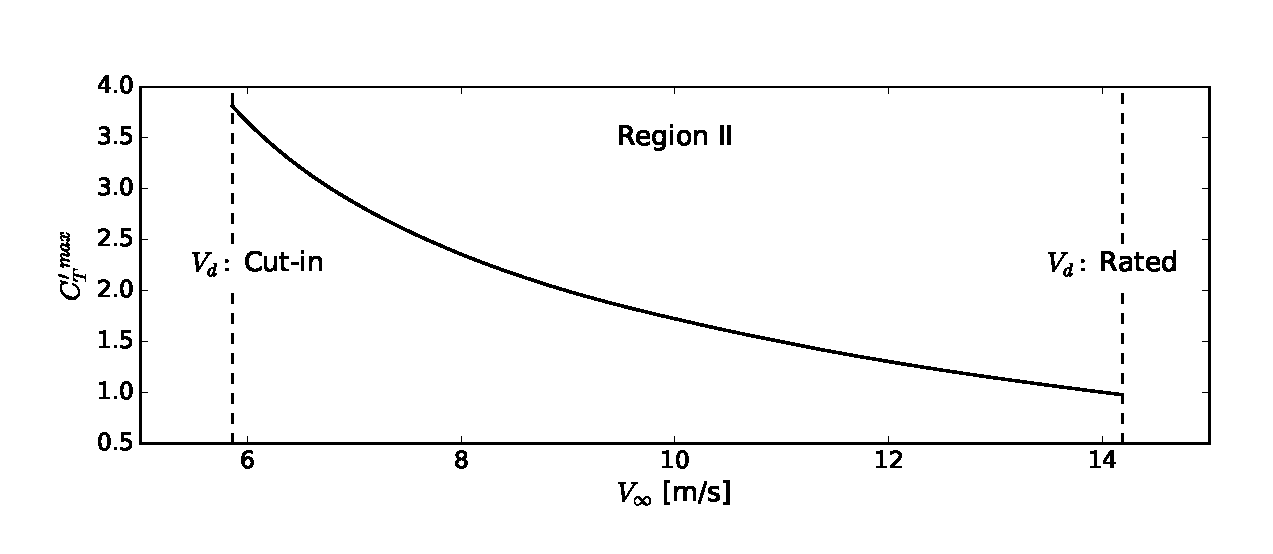
\includegraphics[width=0.9\linewidth]{chapters/methodology/figure7.eps} 	
	\caption{Maximum attainable modified thrust coefficient $C_T'^{max}$ for region II operation of the NREL-5 MW turbine through increase of $\lambda$ as a function of undisturbed upstream velocity $V_\infty$.}\label{fig:Ct_Uinfty}
\end{figure}

\subsubsection{Yaw control}
Turning to the control of the orientation of the thrust force, we affect the yaw angle $\theta_i$ of turbine $i$ by imposing a yaw rate $\omega_i$ as 
\begin{equation}
\ddt{\theta_i} = \omega_i \label{eq:omega_def}.
\end{equation}
Similar to the thrust coefficient, we impose box constraints on the yaw rate as $-\omega_{\text{max}} \leq \omega \leq \omega_{\text{max}}$. Unless stated otherwise, the maximal yaw rate is chosen as $\omega_{\text{max}} = 0.3^\circ/s$, as specified for both the DOWEC 6-MW and NREL 5-MW turbine designs \citep{Kooijman2003, jonkman2009definition}.

\section{Numerical discretization}\label{sec:meth_discr}
The current section discusses the numerical discretization of the governing equations (\ref{eq:NSmomentum}-\ref{eq:NScontinuity}) in the SP--Wind framework. The framework was developed over the years at KU Leuven, and has been applied in DNS and LES studies for simulation and optimization on channel flows \citep{meyers2007evaluation, meyers2007plane,nita2016efficiency}, mixing layers \citep{delport2009constrained, delport2011maximizing}, and wind farm boundary layers \citep{meyers2010large, calaf2010large, allaerts2015large, goit2015optimal, goit2016optimal}.

Firstly, the spatial discretization and associated boundary conditions are discussed. Thereafter, the methods for time integration and pressure-velocity coupling will be discussed. As will be shown, some of the operations resulting from the discretization schemes involve highly non-local computations, which has important consequences for the distributed-memory parallelization of the simulation solver (discussed in Section~\ref{sec:meth_par}). 

\subsubsection{Spatial discretization}
The governing equations are spatially discretized using a Fourier pseudo-spectral method in the horizontal ($x$, $y$) directions, combined with a fourth order energy-conserving finite difference scheme in the vertical ($z$) direction \citep{verstappen2003symmetry}. Figure~\ref{fig:physical_fourier} illustrates the solution field representation in physical space (Figure~\ref{fig:physical_fourier}a) and its modal decomposition in Fourier space (Figure~\ref{fig:physical_fourier}b). The relationship between both can be expressed through the truncated discrete Fourier analysis, i.e. on a discrete $N \times N$ grid:
\begin{align}
%	\ufilt(x, y, z) = \sum_{k_x = -\frac{N}{2} k_{min}}^{(\frac{N}{2} - 1) k_{min}  \sum_{k_y = }^{max} \hat{\bs{u}} (k_x, k_y, z) 
	\ufilt(x, y, z) &= \sum_{k_x = -\frac{N}{2} k^\star_x}^{(\frac{N}{2} - 1) k^\star_x} \sum_{k_y = -\frac{N}{2} k^\star_y}^{(\frac{N}{2} - 1) k^\star_y}    \hat{\bs{u}} (k_x, k_y, z) \exp\bigg( \imath (k_x x + k_y y) \bigg), \label{eq:DFT}
	%	\ufilt(x, y, z) = \sum_{k_x = -\frac{N}{2} k_{min}}^{(\frac{N}{2} - 1) k_{min}  \sum_{k_y = }^{max} \hat{\bs{u}} (k_x, k_y, z) 
%	\hat{\bs{u}} (k_x, k_y, z) &= \frac{1}{N^2} \sum_{x = 0}^{(1-\frac{1}{N})L} \  \sum_{y = 0}^{(1-\frac{1}{N})L}  \ufilt(x, y, z)   \exp\bigg(-\imath (k_x x + k_y y) \bigg), \label{eq:DFT}
\end{align}
with $\imath$ the imaginary unit, $\hat{\bs{u}}$ the complex-valued Fourier coefficient of the Fourier mode with streamwise wavenumber $k_x$ and spanwise wavenumber $k_y$, and $k^\star_{x/y} = 2\pi/L_{x/y}$. Due to the Hermitian symmetry of the Fourier coefficients, i.e. $\hat{\bs{u}}(k_x, k_y, z) = \hat{\bs{u}}(-k_x, -k_y, z)^* $, half of the Fourier-space field is redundant and needs not be stored in memory, as indicated in Figure~\ref{fig:physical_fourier}. Note that spatial derivatives in the spectral directions can be evaluated exactly and without any non-local information since, by Equation \eqref{eq:DFT}, the derivative operators $\partial_{x/y}$ in real space translate to a multiplication with $\imath k_{x/y}$ in Fourier space. 

Although most operations in the flow solver are performed in Fourier space, a transformation to physical space is required for the efficient computation of the non-linear convective terms and spatially localized terms such as the turbine forcing. This transformation involves a two-dimensional (inverse) discrete Fourier Transform, which is implemented in the SP--Wind solver as sequential one-dimensional Fast Fourier Transforms (FFTs) over the spectral directions $x$ and $y$. FFTs are performed using the open-source FFTW library \citep{frigo1997fastest}. Note that the transformations consist of highly non-local operations involving all the discrete wavenumbers / all the physical locations in the direction over which they are performed, and it is crucial for computational performance that all this data resides in local memory. As will be discussed later, this has far-reaching consequences for the distributed-memory parallelization of the solver. Further, potential aliasing errors originating from non-linear terms are eliminated using the 3/2 dealiasing rule \citep{canuto1988spectral}.

\begin{figure}
	\centering
	\includegraphics[width=\linewidth]{chapters/methodology/physicalfourierpng.eps}
	\caption[Planview in the logarithmic region of instantaneous streamwise component of the velocity field for a typical high Reynolds number wall-bounded turbulent flow.]{Planview in the logarithmic region of instantaneous streamwise component of the velocity field for a typical high Reynolds number wall-bounded turbulent flow. The simulation setup corresponds to the precursor simulations used in Chapter~\ref{ch:opt_induction}, further detailed in Table~\ref{tab:setup_params_ind}. \emph{a)} Physical space velocity $\tilde{u}_x (x, y, z=0.1H)$. \emph{b)} Amplitude of Fourier modal velocity $\vert \hat{u} \vert (k_x, k_y, z=0.1H)$ \label{fig:physical_fourier}}
\end{figure}

The horizontal projection of the solution field onto periodic Fourier modes implies that the discrete governing equations are solved on a domain of infinite horizontal extent with periodic boundary conditions at the lateral domain boundaries. However, a so-called fringe region technique can be used in order to impose non-cyclic inflow conditions without breaking global periodicity, further elaborated in Section~\ref{sec:meth_fringe}. Unless explicitly stated otherwise, the top boundary is treated with a stress-free condition, emulating a fixed ABL height at the top of the domain. At the bottom boundary an impermeable wall stress boundary condition is imposed, relating the wall stress to the wall-parallel velocity consistent with log-law behavior at the first gridpoint away from the wall \citep{bou2005scale, calaf2010large}. 


\subsubsection{Time integration}
Time integration is performed using a four-stage fourth-order fully explicit Runge--Kutta method. For the regular large-eddy simulations in this manuscript, the value of the time step is adaptively chosen to be consistent with a maximum Courant--Friedrichs--Lewy (CFL) number of 0.4. The optimal control simulations on the other hand use a fixed constant time step, for which the CFL number fluctuates slightly around 0.4. 

\subsubsection{Pressure-velocity coupling}
As is standard practice in incompressible flow simulations, the coupling between pressure and velocity is obtained by taking the divergence of the momentum equation \eqref{eq:NSmomentum} and enforcing the solenoidal continuity constraint \eqref{eq:NScontinuity}, resulting in the following Poisson equation for pressure: 
\begin{equation}
	\nabla^2 \ptilde = \nabla \cdot \bigg( \sum_{i=1}^{N_t} \blds{f}_i - \nabla \cdot \blds{\tau}_{\text{sgs}} - (\ufilt \cdot \nabla) \ufilt \bigg) \equiv R
\end{equation}

Note that, for a typical finite difference / finite volume flow solver on a $N^3$ grid, discretizing this equation results in a coupled linear system characterized by a sparse $N^3 \times N^3$ matrix with 19 non-zero entries per row for the aforementioned fourth-order finite difference scheme. Solving this linear system is often the most expensive step in an explicit flow solver. However, due to the spectral discretization in horizontal directions considered here, the system can be decoupled per wavenumber pair ($k_x, k_y$):
\begin{align}
	(-k_x^2 - k_y^2) \hat{p} + \partial^2_z \hat{p} &= \hat{R}\label{eq:poisson_decoupled}
\end{align}

It is important to note that the discretization of Equation \eqref{eq:poisson_decoupled} leads to a relatively small linear system characterized by a sparse banded $N \times N$ matrix with a bandwidth of 7 for each of the $N/2 \times N$ wavenumber pairs (factor 2 because of Hermitian symmetry described above). This offers great opportunity for efficient parallelization: provided that each processor has the full $z$ direction in local memory, each discretized Poisson system can be solved easily using standard methods. In the SP--Wind framework each system is solved using a direct LU-based solver. The total workload in the form of $N/2 \times N$ independent linear systems is distributed across several processes requiring no communication.

\section{Inlet boundary conditions}\label{sec:meth_fringe}
In our pseudo-spectral LES method, the inherent cyclic boundary conditions are circumvented in the streamwise direction ($x$) through the use of a \emph{fringe region} technique \citep{spalart1993experimental,lundbladh1999efficient,nordstrom1999fringe}. In this technique, flow variables are smoothly forced to desired inflow values by adding a body force to the governing equations in a so-called ``fringe region'' at the back of the domain. This allows the entire field to stay periodic while the region of interest (the domain minus the fringe region) is non-periodic.

The fringe force penalizes the error between actual field variables $\ufilt$ and their desired inflow values $\bs{u}_\text{in}$ in the fringe region, and is constructed here as:
\begin{equation}\label{eq:fringeforcing}
	\bs{f}_{\text{fr}}(\bs{x}) =  - \lambda(x) \bigg(\ufilt(\bs{x}) - \bs{u}_{\text{in}}(\bs{x})  \bigg),
\end{equation}
with a one-dimensional fringe force masking function $\lambda$ defined as \citep{lundbladh1999efficient}
\begin{align}
\lambda(x) &= \lambda_{max} \bigg \{ \mathcal{S}\left( \frac{x - x_s}{\Delta_s} \right) - \mathcal{S} \left( \frac{x - x_e}{\Delta_e} + 1 \right) \bigg \} \nonumber,\\
\mathcal{S}(x) &=
\begin{cases}
0                  & x \le 0        \\
1/[1 + \exp(\frac{1}{x-1} + \frac{1}{x})]             & 0 < x < 1   \\
1                        & x \ge 1 .  \\
\end{cases} \label{eq:lambda}
\end{align}
The masking function is non-zero only inside the fringe region part of the domain. A smooth and infinitely differentiable combination of exponentials defined in \eqref{eq:lambda} avoids the introduction of any jump discontinuities, and is therefore amenable to spectral methods without causing spurious Gibbs oscillations. The parameters $x_s$ and $x_e$ set the start and end of the fringe region, while $\Delta_s$ and $\Delta_e$ provide control over the smoothness of the fringe masking function. Figure~\ref{fig:lambda} illustrates a masking function with typical parameters. The maximum value of the masking function $\lambda_{max}$ is chosen to be high enough to provide sufficient damping of the flow solution in the fringe region, yet low enough to satisfy the stability constraint $\lambda_{max}\Delta t \le 2.78$ for 4th order explicit Runge-Kutta time integration \citep{schlatter2005windowing} without the need to decrease the time step. Typical values used for the simulations in this work range from $\lambda_{max} = 1 500$ to $3 000$ for time steps of the order of $5 \times 10^{-4} H/u_*$. The localized fringe forcing results in a distortion of the flow field and its dynamics inside the fringe region. However, the influence of this forcing on flow dynamics in the domain of interest outside the fringe region has been shown to be small \citep{nordstrom1999fringe}.

The inflow conditions $\bs{u}_{\text{in}}$ in \eqref{eq:fringeforcing} themselves can consist of e.g. simple uniform inflow, synthetic turbulence, or coherent turbulence obeying the Navier--Stokes equations. The generation of turbulent inflow is further elaborated in Chapter~\ref{ch:turbulent_inflow}. 

\begin{figure}[t]
	\centering
	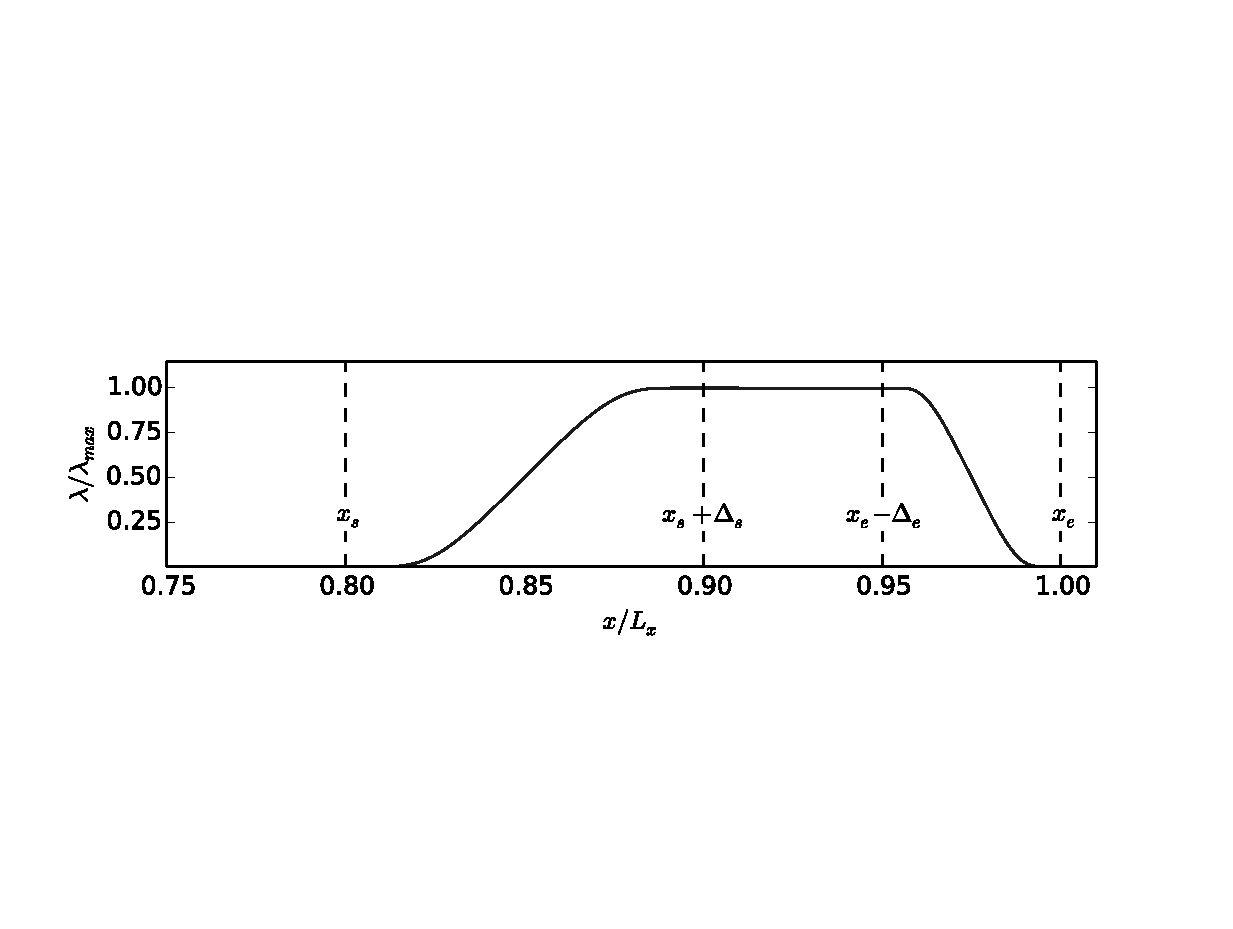
\includegraphics[width = \textwidth,trim= 0cm 4.4cm 0cm 5cm,clip]{chapters/methodology/lambda_fringefunction.eps}
	\caption[Example of a fringe masking function $\lambda(x)$.]{Example of a fringe masking function $\lambda(x)$, defined by Equation \eqref{eq:lambda}, with parameters $x_{s} = 0.8L_x$, $x_{e} = L_x$, $\Delta_{s} = 0.1L_x$ and $\Delta_{e} = 0.05L_x$.}
	\label{fig:lambda}
\end{figure}	



\section{Solver parallelization}\label{sec:meth_par}
Due to the large amount of degrees of freedom ($10^{10} - 10^{14}$ combined in space and time) present in typical simulations performed by the SP-Wind platform, a highly scalable parallelization strategy is a prerequisite for performing simulations in a timely manner. To this end, the simulation solver uses distributed-memory parallelism through the MPI message passing interface, which can scale up to thousands of processors. With MPI, data and computational loads are divided among a set of MPI processes running in their individual memory address space. Throughout the following discussion, we presuppose that each MPI process is bound to a single dedicated processor core, as is standard practice in scientific computing. Sets of MPI processes can be grouped together into so-called MPI communicators. For instance, the standardly-defined communicator $\verb|MPI_COMM_WORLD|$ refers to the set of all processes running an instance of the MPI-parallel program.

The main advantage of distributed-memory parallelism is its scalability up to thousands of cores on any modern high-performance computing (HPC) system. The downside however is
that data contained on the simulation grid is partitioned over the processes, and that communication is required at several points throughout the
simulation. As mentioned before, a judicious choice of the grid partitioning topology however can limit the total amount of required communications.
Previous optimization studies using the SP--Wind solver applied a slab decomposition strategy with limited scalability \citep{delport2009constrained,
goit2015optimal}. This has led to excessive turnaround times for performing optimal control simulations, i.e. the control of a fully-developed
wind-farm boundary layer over a physical timespan of $\approx$ 1 hour involved a total wall time of over 70 days \citep{goit2015optimal}, entailing to
a physical to computational time ratio of approximately 1: 1800. To reduce the time-to-solution and thus accelerate the solver, a new state of the art
pencil decomposition method has been implemented in the context of the current work \citep{li20102decomp}. It will be shown later that this, in
combination with the upgraded optimization algorithms implemented within this thesis, has led to better converged optimal control results obtained in
a physical to computational time ratio of about 1:700 (when running on 320 Ivy Bridge processor cores).

Section~\ref{sec:meth_par_part} discusses both new and previous grid partitioning strategies and resulting communication patterns used in the solver. In addition, a strong scaling test illustrates the excellent scalability of the new strategy. Thereafter, Section~\ref{sec:meth_par_map} shows that, by taking into account the topology of HPC hardware when binding processors to certain parts of the domain, parallel scaling can be improved by a significant amount.

\subsection{Simulation grid partitioning}\label{sec:meth_par_part}
Figure~\ref{fig:grid_partitioning} illustrates the strategies for decomposing the global simulation domain into local domains available in the SP--Wind solver, i.e. a one-dimensional slab decomposition and a two-dimensional pencil decomposition. The current section further elaborates on the advantages and disadvantages of both and shows a performance comparison for a numerical setup relevant to the simulations performed in this dissertation. 

\begin{figure}
	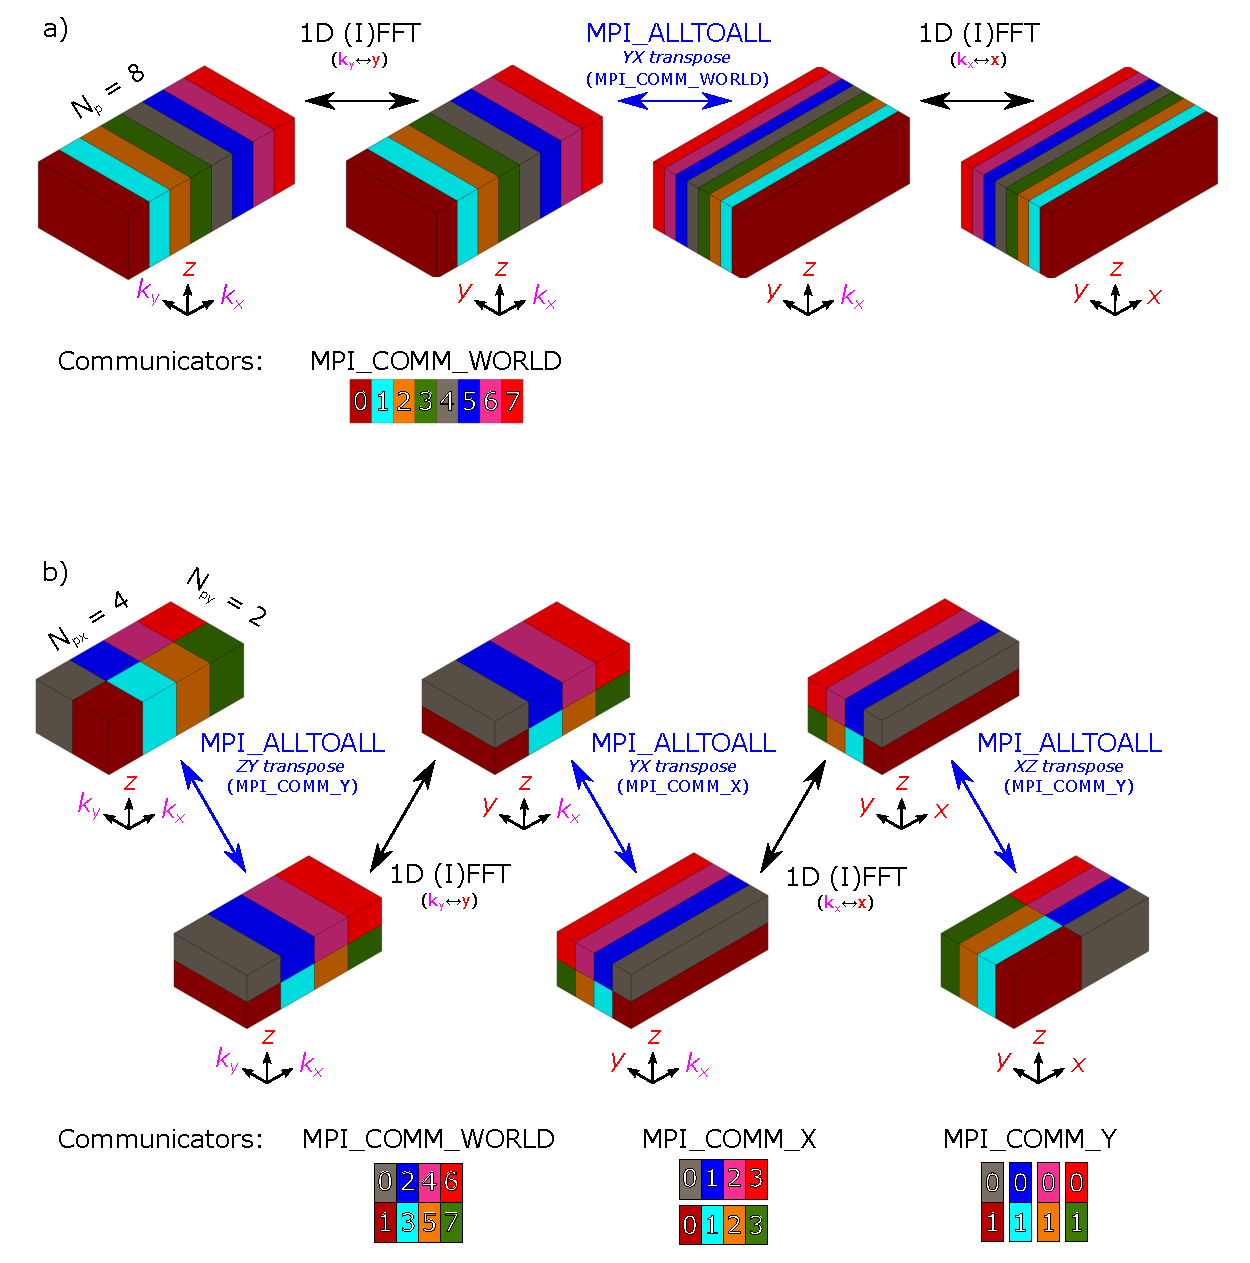
\includegraphics[width=\textwidth]{figures/meth_slab_pencil.eps}
	\caption[Simulation grid partitioning and associated communication patterns during two-dimensional (inverse) Fourier transforms.]{Simulation grid partitioning and associated communication patterns during two-dimensional (inverse) Fourier transforms. \emph{a)} One-dimensional slab decomposition with $N_p = 8$. \emph{b)} Two-dimensional pencil decomposition with $N_p = 8$, $N_{px} = 4$, and $N_{py} = 2$. \label{fig:grid_partitioning}}
\end{figure}

\subsubsection{Slab decomposition} 
Figure~\ref{fig:grid_partitioning}a depicts the classical one-dimensional slab decomposition used in previous studies \cite{delport2009constrained, calaf2010large, goit2015optimal}. The figure illustrates the decomposition of the domain over 8 MPI processes. Throughout the simulation, the entire spatial simulation grid is distributed along a single dimension, while the other two are kept local within a processor core. As shown in the figure, this results in slab-shaped cuts of the global domain. As mentioned above, when transforming between physical and wavenumber space, it is crucial that the full axis along which a FFT is performed resides in local memory. Furthermore, in order to keep the evaluation of derivatives in the convective terms and the solution of the Poisson equation as efficient as possible, the vertical finite difference direction is kept local as well in both physical and Fourier space. Starting from the latter Fourier space, the domain is divided into so-called $yz$ slabs, with both the $y$ and $z$ directions in local memory, and is distributed along the $x$ axis.  In order to perform a two-dimensional FFT along the $x$ and $y$ directions, a distributed array transpose is required between the consecutive one-dimensional FFTs. This requires a so-called \emph{all-to-all} communication, in which every process both sends and receives data to and from all other processes within a given communicator. As shown in the figure, this all-to-all communication is performed over the set of all processes involved in the program, i.e. the $\verb|MPI_COMM_WORLD|$ communicator, and leads to a transposed partitioning in the form of $xz$ slabs in physical space. 

Note that, due to the one-dimensional decomposition, the maximum amount of cores that can be used is limited to the smallest amount of gridpoints in the horizontal directions, i.e $N_{p,\text{max}}^{\text{slab}} = \min(N_x, N_y)$. Furthermore, all communications between processes are performed in a single global all-to-all step. Since the amount of messages exchanged in such an operations scales quadratically with the total amount of involved processes, the communication cost of the slab decomposition strategy is hence proportional to $N_p^2$.

\subsubsection{Pencil decomposition} 
Figure~\ref{fig:grid_partitioning}b shows a two-dimensional pencil decomposition. This type of decomposition is the current state of the art method for parallel spectral simulation tools, as indicated by the availability of open-source libraries such as P3DFFT \citep{pekurovsky2012p3dfft} and 2DECOMP\&FFT \citep{li20102decomp}. In contrast to the previously described slab approach, the domain is distributed along two directions and data locality is only preserved in one, resulting in a pencil-shaped local domain cut. As for the slab decomposition, both the calculation of vertical derivatives in the nonlinear terms in real space and the Poisson equation solve in Fourier space are preferably performed in local domains with data locality in the $z$ direction, i.e. by using $z$ pencils. Furthermore, the efficient calculation of the consecutive one-dimensional FFTs requires the grid to be partitioned as $x$ and $y$ pencils as shown in the figure, resulting in a three-step communication pattern. Note that, in contrast to the slab decomposition described above, each communication step however uses an all-to-all communication which involves only a subset of the global $\verb|MPI_COMM_WORLD|$ communicator, indicated by $\verb|MPI_COMM_Y|$ (ZY and XZ transpose over $N_{py}$ processes) and $\verb|MPI_COMM_X|$ (YX transpose over $N_{px}$ processes). The division of the total amount of processes $N_p$ over these communicators provides an additional degree of freedom. 

The maximum amount of cores that can be utilized in the current approach is $N_{p,\text{max}}^{\text{pencil}} = \min(N_x \times N_y, N_x \times N_z, N_y \times N_z)$. For simulation grids relevant in the context of this thesis, this leads to $N_{p,\text{max}}^{\text{pencil}} \approx 10^4 - 10^5$, which exceeds the full capacity of most present-day Tier 2 and Tier 1 supercomputing infrastructures. A first communication cost estimate can be made on the amount of exchanged messages in the sequential all-to-all steps. Assuming parallel all-to-alls in independent communicators do not interact, this estimate is $N_{px}^2 + 2N_{py}^2$ (note that this assumption is not strictly true in practice). According to this reasoning, the optimal distribution would approximate a ratio of $N_{px}/N_{py} \approx \sqrt{2}$, albeit with $N_{px}$ and $N_{py}$ integers. However, we will show later that the topology of the hardware infrastructure can be utilized to obtain more favorable process distributions with lower communication costs. Finally, note that the slab decomposition from previous paragraph can be regarded as a special case of a pencil decomposition, i.e. with $N_{px} = N_p$, and $N_{py} = 1$. 

%Depending on whether or not the parallel alltoalls within a step affect one another, this estimate is $N_{py} N_{px}^2 + 2 N_{px} N_{py}^2$ or $N_{px}^2 + 2N_{py}^2$ respectively. According to this reasoning, the optimal distribution would approximate a ratio of $N_{px}/N_{py}$ between $\sqrt{2}$ and 2, albeit with $N_{px}$ and $N_{py}$ integers. However, we will show later that the topology of the hardware infrastructure can be utilized to obtain more favorable process distributions with lower communication costs. 

\subsubsection{Performance comparison}
Figure~\ref{fig:strongscaling} shows the performance of aforementioned grid partitioning strategies, based on benchmark results of a strong scaling test. The test is performed on the 2016 Flemish Tier1 supercomputer BrENIAC, equipped with compute nodes containing two Intel Xeon E5-2680v4 processors (2.4GHz, 14 cores per processor, Broadwell architecture) which are interconnected by a high-bandwidth and low-latency EDR Infiniband network. The scaling test is performed for a canonical high Reynolds number half-channel flow, using a simulation grid of $512 \times 256 \times 256 \approx 33.5 \times 10^6$ grid points. As a consequence, the maximum amount of cores on which a slab decomposition can be performed is $N_p^{\text{slab}} = N_y = $ 256 processor cores. In contrast, a pencil decomposition allows simulations to be performed up to a maximum of $N_p^{\text{pencil}} = N_y \times N_z = 65~536$ cores. Even for this standard grid size, this theoretical maximum exceeds the total amount of cores on the BrENIAC supercomputer by a factor of four. For practical reasons, the performance of the pencil decomposition strategy is tested up until 1 334 cores, i.e. 48 full compute nodes. 

Figure~\ref{fig:strongscaling}a shows the wall time per time step as a function of the amount of processors, which is a measure for the absolute computational cost in terms of time-to-solution. It can be seen from the figure that, for the test conducted here, the pencil decomposition allows to reduce the wall time by approximately an order of magnitude compared to the best slab decomposition run. Furthermore, the slope of the pencil decomposition curve deviates only slightly from the ideal curve for the largest amount of processors, suggesting that, on larger machines, wall time could be even further reduced by increasing the core count. However, this deviation from the ideal linear scaling slope, albeit relatively small, indicates that communication overhead starts to play an important role for a large amount of cores. Figure~\ref{fig:strongscaling}b shows the parallel efficiency, defined as the ratio between the ideal wall time per time step assuming perfect linear scalability on the one hand, and the actual wall time per time step for a given amount of cores on the other. The reference value for the computation of parallel efficiency is one full compute node, i.e. with 28 MPI processes. In contrast to the wall time shown in Figure~\ref{fig:strongscaling}a, the parallel efficiency in Figure~\ref{fig:strongscaling}b is a measure for computational cost in terms of CPU-hours. Also shown in the figure is the red dot-dashed line indicating a parallel efficiency of $70\%$, which is often used as a rule of thumb guideline for an acceptable parallel execution. It can be seen that for simulations on a small amount of processor cores ($N_p < 48$) the pencil decomposition performs at a lower efficiency than its slab decomposition counterpart. This can be explained by the fact that eliminating the $\verb|MPI_COMM_Y|$ communicator by having a single centralized $\verb|MPI_COMM_WORLD|$ all-to-all communication outweighs the detrimental effects of having a larger $\verb|MPI_COMM_X|$ communicator. However, as the number of processor cores increases, a significant drop in parallel efficiency for the slab decomposition is observed due to the large cost of the blocking collective all-to-all collective communication in which all processes participate. Pencil decompositions on the other hand allow to convert the single large all-to-all communication step into 3 smaller all-to-alls. This not only reduces the size of the blocking all-to-all communications, but also improves concurrency by allowing them to be executed in parallel without blocking all processes collectively. Figure~\ref{fig:strongscaling}b indicates that, by doing so, the sharp decline in parallel efficiency can be mitigated up until a much larger core count. 

\begin{figure}
	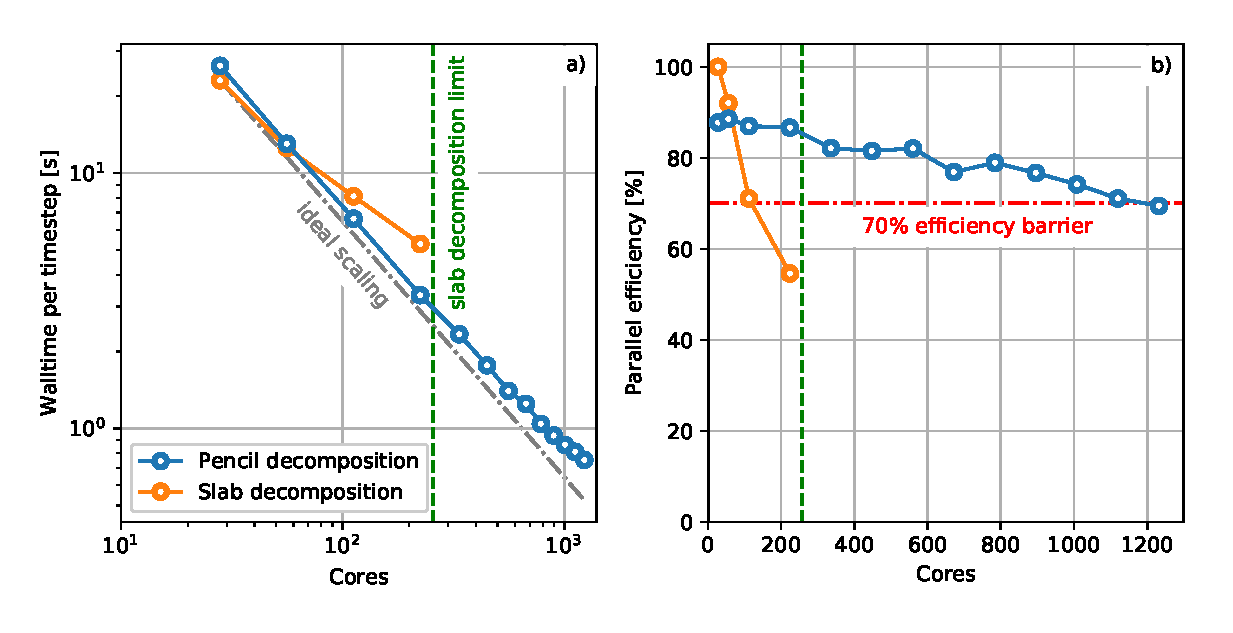
\includegraphics[width=\textwidth]{figures/meth_strong_scaling.eps}
	\caption[Strong scaling plot for SP-Wind solver using a grid with $512 \times 256 \times 256$ grid points.]{Strong scaling plot for SP-Wind solver using a grid with $512 \times 256 \times 256$ grid points. \emph{a)} Walltime per time step within Runge-Kutta time integration. \emph{b)} Parallel efficiency in comparison to single-node slab decomposition. The dashed green line indicates the maximum amount of processor cores on which a solver with a slab decomposition can run.\label{fig:strongscaling}}
\end{figure}

\subsection{Processor mapping \& intranode communication}\label{sec:meth_par_map}

As mentioned above, a pencil decomposition provides an additional degree of freedom in the form of how to distribute the total amount of processors $N_p$ in the $\verb|MPI_COMM_WORLD|$ communicator into subcommunicators $\verb|MPI_COMM_X|$ and $\verb|MPI_COMM_Y|$, containing $N_{px}$ and $N_{py}$ processors respectively, with $N_p = N_{px} \times N_{py}$. A well-reasoned choice for this distribution has already been mentioned above, i.e. the cost estimate based on the amount of exchanged messages can be minimized by approximating the ratio $N_{px}/N_{py} \approx \sqrt{2}$. This strategy will be referred to as a `balanced' distribution in the remainder of this discussion, as it aims to balance the cost of all communication steps throughout the code. 

Alternatively, one could abandon the aim of balancing all communications and focus on minimizing the cost of either the $\verb|MPI_COMM_X|$ or the $\verb|MPI_COMM_Y|$ steps by exploiting the hardware topology. On modern HPC infrastructure, MPI communication between processes residing on the same computational node (\emph{intranode} communication) can be performed at a significantly lower cost than communication that has to go over the interconnect network between different nodes (\emph{internode} communication). Hence, for the given cluster with 28 cores per node, we can exploit this by judiciously mapping process ranks to selected cores, and choosing $N_{px} = 28$ or $N_{py} = 28$ in order to obtain either intranode $\verb|MPI_COMM_X|$ or intranode $\verb|MPI_COMM_Y|$ communicators. As shown in Figure~\ref{fig:grid_partitioning}b, this either results in an intranode YX transpose (for intranode $\verb|MPI_COMM_X|$), or in intranode ZY and XZ transposes (for intranode $\verb|MPI_COMM_Y|$). 

\begin{figure}
	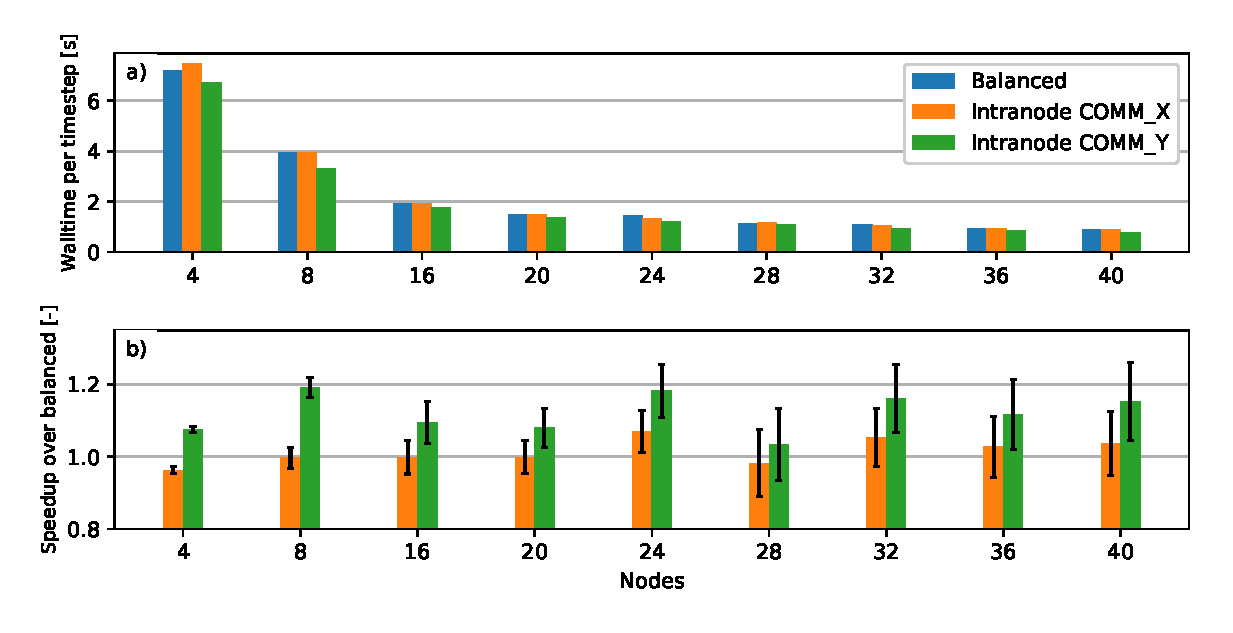
\includegraphics[width=\textwidth]{figures/meth_balanced_intranode.eps}
	\caption[Performance of processor distribution strategies for a pencil decomposition.]{Performance of processor distribution strategies for a pencil decomposition. \emph{a)} Walltime per time step. \emph{b)} Speedup of intranode strategies over  balanced distribution. Errorbars indicate a 95$\%$ confidence interval. \label{fig:balanced_intranode}}
\end{figure}

Figure~\ref{fig:balanced_intranode} illustrates the performance of the abovementioned approaches on a wide range of node counts. As shown in Figure~\ref{fig:balanced_intranode}b, a significant overall speedup in the order of $10 - 20\%$ can be achieved when choosing intranode $\verb|MPI_COMM_Y|$ communicators over a balanced processor distribution. This is not the case for intranode $\verb|MPI_COMM_X|$ communicators: the increased cost of internode $\verb|MPI_COMM_Y|$ communication seems to annul the intranode cost reduction. The results presented here indicate the importance of considering both code characteristic and hardware topology when optimizing code scalability. All further simulations throughout this work apply pencil decomposition parallelism with intranode $\verb|MPI_COMM_Y|$ communicators.

\section{Summary}
The current chapter elaborated on the evaluation of the wind-farm boundary layer state and the wind-farm power extraction using large-eddy simulations. The governing equations were introduced, and the associated discretization schemes have been elucidated. Furthermore, requirements for data locality for different operations in solving the equations were indicated. Further, the upgrade in the solver parallelization scheme from a slab decomposition to a pencil decomposition strategy was illustrated, and excellent scalability was demonstrated. In addition, the importance of taking into account hardware topology when optimizing code performance was shown.  As will be evidenced throughout this text, the speedup achieved through this parallelization upgrade facilitates more and better converged optimal control simulations. 

In addition to the in-house SP--Wind framework described in the current chapter, several free and open-source software tools were employed for the analysis and visualization of simulation results reported throughout this thesis. More specifically, the author would like to acknowledge the developers of the VAPOR visualization software \citep{vapor}, and of the Numpy \citep{numpy}, matplotlib \citep{matplotlib}, and scikit-learn \citep{scikit-learn} Python software packages. 

This chapter also introduced the implementation of a fringe region technique to allow the simulation of non-periodic and spatially-developing wind-farm flows using the Fourier pseudo-spectral SP--Wind framework. However, a key element in performing turbulence-resolving simulations of non-periodic flows is the generation of unsteady and coherent turbulent inflow conditions. This will be elaborated in detail in the following chapter. 

%%%%%%%%%%%%%%%%%%%%%%%%%%%%%%%%%%%%%%%%%%%%%%%%%%
% Keep the following \cleardoublepage at the end of this file, 
% otherwise \includeonly includes empty pages.
\cleardoublepage

